\documentclass[11pt]{article}

\usepackage{graphicx}
\usepackage{multirow}
% make text wrap a figure
\usepackage{wrapfig}
% a package against words hyphenation. Perhaps, it works
\usepackage[none]{hyphenat}
\usepackage{eurosym}
\usepackage{textcomp}
\usepackage{amsmath}
% change the date format (avoid printing the day of week in the \today command)
\usepackage[ddmmyyyy]{datetime}
% control headers and footers
\usepackage{fancyhdr}
\usepackage[usenames, dvipsnames]{color}

% date separator
\renewcommand{\dateseparator}{.}

\definecolor{myGray}{gray}{0.15}

\usepackage{ifpdf}
\ifpdf
\usepackage[pdftex, colorlinks=true, urlcolor=myGray]{hyperref}
\else
\usepackage[hypertex]{hyperref}
\fi

\textheight = 680pt
%\textheight = 640pt
\hoffset = -35pt
\textwidth = 450pt
\voffset = -50pt

% header and footer
\pagestyle{fancy}
\fancyhead[L]{\textit{Ivan Martynov / +358 44 936 6589/
\href{ivan.a.martynov@gmail.com}{ivan.a.martynov@gmail.com}}}
\fancyhead[R]{\textit{\thepage}}
\fancyfoot{}

\newcommand{\xfill}[2][2.5pt]{\dimen0=#2\advance\dimen0 by #1  \leaders
\hrule height \dimen0 depth -#1\hfill}
\newcommand{\sectitle}[1]{\MakeUppercase{\bf\,\xfill{0.25mm}\,#1}\,
\xfill{0.25mm}\phantom{\ }\\\smallskip}

% solution for C# sign
\newcommand{\Csharp}{%
  {\settoheight{\dimen0}{C}C\kern-.05em \resizebox{!}{\dimen0}{\raisebox{\depth}{\#}}}}

% two solutions for C++ sign
%\newcommand{\CC}{C\nolinebreak\hspace{-.05em}\raisebox{.4ex}{\tiny\bf +}\nolinebreak\hspace{-.10em}\raisebox{.4ex}{\tiny\bf +}}
\def\CC{{C\nolinebreak[4]\hspace{-.05em}\raisebox{.4ex}{\tiny\bf ++}}}

\begin{document}

\begin{table}
  \begin{tabular}{p{200pt} p{120pt} p{150pt}}
    & & \multirow{7}{*}{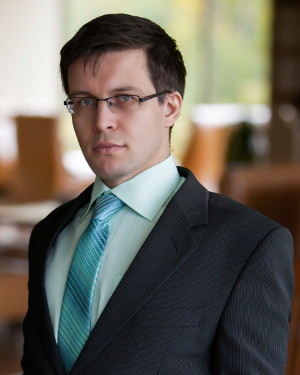
\includegraphics[width=85pt]{me_2013_09.png}}\\
    \textbf{Ivan Martynov} & \textbf{CV} &\\
    & \today &\\
    53810 Lappeenranta & &\\
    phone +358 44 936 6589& &\\
    \href{ivan.a.martynov@gmail.com}{ivan.a.martynov@gmail.com} & &\\
    Born 12.04.1982, Petrozavodsk & &\\
    Citizenship: Finland, Russia & &
  \end{tabular}
\end{table}

%---------------------------------------------------------------------------

\noindent
\sectitle{expertise}
\vspace{-20pt}
\begin{itemize}
  \setlength\itemsep{1pt}
  \item Programming languages: C/\CC/\Csharp, Python, Java, \LaTeX
  \item Programming concepts: OOP, image processing, computer graphics
  \item Research (mathematics, image processing)
    % \item Driving (class B and own car)
\end{itemize}

\begin{flushleft}

  \sectitle{employment history}

  \textbf{Software programmer, CISS Software Oy, Oct.\,2021 --}\\
  Implementing CAD applications features and code maintenance.
  \medskip

  \textbf{Software engineer, Finnos Oy, Oct.\,2016 -- Aug.\,2020}\\
  Algorithm development for the log sorting system. Devising and
  implementing methods for calculation of geometrical features of timber logs
  and their sawing patterns. Visualizing results in 2D and 3D.\\
  \medskip

  \textbf{Project manager, SMIF Oy, Sep.\,2012 -- Sep.\,2013}\\
  %  \textit{The company was established in 2011 as a daughter company of Russian company TKA with the intention to extend the activity of the latter to the  European region.}\\
  Control of web-site development, paper work and other tasks.\\
  \medskip

%  \newpage

  \textbf{Younger researcher, Lappeenranta-Lahti University of Technology,
  May.\,2010 --
    April.\,2011}\\
  Research at Machine Vision laboratory. The project's primary focus was the use of structured light patterns for a 3D reconstruction of an object's shape.
  I have been actively using the Matlab software and C++ programming
  language under Linux operating system.\\
  \medskip

  \textbf{Engineer of an Internet class,  Internet company ``Sampo.ru'',
  Petrozavodsk,\\Jun. -- Aug.\,2007 and Jun. -- Aug.\,2006 (tot. 6 months)}\\
  %  \textit{The company is an Internet provider in Petrozavodsk.}\\
  Working with customers, cash register and performing varying
  office work. Assisting users in an
  Internet class. Making agreements with
  customers for providing Internet to their homes.\\
  \bigskip

  %------------------------------------------------------------------------------

  \sectitle{education}

  \textbf{Ph.\,D., Lappeenranta University of Technology, 2012 --}\\
  \textit{Major subject:} image processing, shadow detection.\\
  \medskip

  \textbf{Master of Science, Lappeenranta-Lahti University of Technology,
    2006 -- 2008}\\
  \textit{Degree program:} information technology; \textit{major subject:}
  technomathematics, \textit{minor subject:} information technology.\\
  Master's thesis: Computing the persistent homology of range images with alpha
  shapes.\\
  \medskip

  \textbf{Master of Science, Petrozavodsk State University, 2002 -- 2008}\\
  \textit{Degree program:} mathematics; \textit{major subject:} topology,
  \textit{minor subject:} mathematics.\\
  Master's thesis: About free products homeomorphisms.\\
  \bigskip

  \newpage

  \textbf{Coursera.org courses (no certificate):}\\
  \vspace{-10pt}
  \begin{itemize}
    \setlength\itemsep{-3pt}
    \item Game Design: Art and Concepts Specialization (four courses)
    \item Introduction to Interactive Programming in Python (two parts)
    \item Introduction to Game Development (introducing to Unity)
    \item Python for Everybody (four courses)
    \item Java Programming (two courses)
  \end{itemize}

  %------------------------------------------------------------------------------


  \sectitle{language skills}

  \begin{table}[h]
    \begin{tabular}{l l}
      \textbf{Finnish:} good (upper intermediate level certificate, B2-C1) &
      \textbf{French:}  basics\\
      \textbf{English:} excellent (using actively since 2006) &
      \textbf{Russian:} mother tongue
    \end{tabular}
  \end{table}

  %------------------------------------------------------------------------------

  \sectitle{it skills}

  \begin{table}[h]
    \begin{tabular}{l l}
      \textbf{Operation systems:} & Windows, Linux (excellent), Mac OS X (basics)\\
      \textbf{Software:} & Office tools (Microsoft and LibreOffice), Visual
      Studio (.NET, Code),\\
                         & CAD (Microstation), Graphics (Inkscape, Gimp, Krita),\\
      \textbf{Programming:} & C/\CC/\Csharp, Python, Java, \LaTeX
    \end{tabular}
  \end{table}

  %------------------------------------------------------------------------------

  %  \sectitle{additional activities}
  %
  %  \begin{table}[h]
  %    \begin{tabular}{p{107pt} p{300pt}}
  %      \textbf{8\,--\,10 Jun 2009} & 16$^\text{th}$ International Summer School
  %        in Novel Computing, courses:\\
  %      \textbf{10\,--\,14 Aug 2009} & \emph{Scientific Writing} and
  %      \emph{Speaker and Language Recognition}\\
  %      \textbf{9\,--\,13 Aug 2010} & 17$^\text{th}$ International Summer School
  %        in Novel Computing, course:
  %      \emph{Vision for Robotic Localization and Mapping}\\
  %      \textbf{8\,--\,11 Aug 2011} & 18$^\text{th}$ International Summer School
  %      in Novel Computing, course:
  %      \emph{Fuzzy Clustering for Image Segmentation}\\
  %      \textbf{30 Sep\,--\,4 Oct 2013} & Workshop on Computational and Modelling
  %        Problems from Industry, problem:
  %      \emph{Modelling of the electrohydraulic device}\\
  %      \textbf{9\,--\,13 Jun 2014} & The 18$^\text{th}$ European Conference on
  %        Mathematics for Industry\\
  %      \textbf{23\,--\,29 Sep 2015} & 13$^\text{th}$ International Conference of
  %        Numerical Analysis and Applied Mathematics
  %    \end{tabular}
  %  \end{table}
  %

  %------------------------------------------------------------------------------

  \sectitle{personal qualities}

  Communicative, responsible, team worker, computer literate, high analytical
  skills, quick learner, strong interpersonal skills, adaptable\\
  \bigskip

  %\textbf{INTERESTS}\\\smallskip
  %Sport (both physical and intellectual), cooking, constructive toys. I like
  %watching movies in English, dancing (break-dance and salsa). I am a blood
  %donor since April, 2012.\\\ \\

  \sectitle{references}
  \textbf{Jere Heikkinen} / \textit{Finnos Oy} / CEO, jere.heikkinen [at] finnos.fi, +358 44 336 8652\\\smallskip
  \textbf{Tuomo Kauranne} / \textit{Lappeenranta-Lahti University of Technology,
  Mathematics and Physics department} / adj. prof., lecturer, tuomo.kauranne
  [at] lut.fi, +358 40 530 0622\\\smallskip
  \textbf{Matylda Jablonska-Sabuka} / \textit{Lappeenranta-Lahti University of
  Technology, Mathematics and Physics department} / post-doctoral researcher,
  matylda.jablonska-sabuka [at] lut.fi, +358 40 531 3041

\end{flushleft}

\end{document}
